%---------------------------------------------------------------------------------------------------
% Design
%---------------------------------------------------------------------------------------------------
\newpage
%\part{Anfang}
\chapter{Design}
\label{cap:Design}

The components resulting from the analysis chapter will now be described here. The Civitas project is split into three parts, an Android app, the back-end, and the Web app. Using BaaS combines these parts and blurs the borders. Due to its out-of-the-box pattern, implementing features to the Android app also effects the back-end and the web app subtly. Hence, the developer has no direct impact on the design of the back-end and the web app. So, one can argue about where to describe them, within design or realization chapter. However, the description will take place in this chapter in the Backendless section. Visualization tools guide a common way to explain software applications. \textit{"UML Diagram is ideal for software developers and program managers who need to illustrate and interpret software application relationships, actions, and connections using the Unified Modeling Language (UML) notation. It works in the following fields:
\begin{itemize}
\item UML Use Case Diagrams
\item UML Sequence Diagrams
\item UML Activity Diagrams
\item UML Class Diagrams
\item ..."
\end{itemize} 
} \cite{uml}


\section{Application Fundamentals}
Consulting the Android Developers website one can find out everything to \textit{"build anything on Android"} \citep{androidDeveloper}. Exploring the app basics within the docs section points out certain key elements for Android apps in general and the Civitas app in particular: Manifest, Permissions, Activities, Intents, Dependencies, Application class, Gradle, and Resources. To not exceed the limits of this study, only the mentioned elements and their direct relatives will be briefly introduced. 

The root of every Android project is the \textbf{Manifest}. Its name must be \textbf{AndroidManifest.xml} and it is mandatory to declare the app's package name, the app components, the app permissions, and the hard- and software features the app requires. Within the Civitas project, the app components and the permission are of particular interest.

Stated in the Manifest, the \textbf{Permissions} are used to deal with sensitive user data. \textit{"Every Android app runs in a limited-access sandbox. If an app needs to use resources or information outside of its own sandbox, the app has to request the appropriate permission."} \ref{permissionRequest} If the app will, e.g. access the device camera, one has to ask the user for the usage at runtime explicitly. 
The Civitas app needs the user permission for the internet connection, location, audio recording, camera, and storage access.
Denying one or more of this permissions leads to limited usability. 

An application is built to interact with the user. \textbf{Activities} are the frame where the interaction takes place. \textit{"In Android developer lingo, an \textit{activity} is one "screenful" of components. Each Android application can contain many activities. For example, an app's initial activity might be a login screen. After the user logs on, Android covers the entire login activity with another, more interesting activity."} \citep[p. 98]{Burd:2017}

A close relative to the activity is called \textbf{fragment}. \textit{"Fragments are like reusable components or subactivities. Likewise to the activity, it controls parts of the screen, and can be reused between screens. This means we can create a fragment for a list of workouts, and a fragment to display the details of a single workout."} \citep[p. 342]{Griffiths:2017}
Exchanging workouts with artefacts leads to the desired extension of this app.

Talking about activities and fragments, one has to consider the communication between them. This is where \textbf{intents} and \textbf{bundles} comes into play. One can append several informations, e.g. about origin and destination to an intent and start a new activity with it. The new activity filters the appended information and follows the desired route. One has to separate between \textbf{explicit} and \textbf{implicit intents}. 
The first sort is used, if one tells Android explicitly which class it should run. Listing \ref{code:explicit_intent} displays how the transition from \textbf{MainActivity} to \textbf{MapActivity} is done.

\fbox{
\lstinputlisting[label={code:Explicit_intent} ,caption={Explicit intent},captionpos=b, style=MeinStyle, numbers = left]{program/design_explicit_intent.java}
}

Line one \textbf{getActivity()} is used, because the intent is initialized within a fragment, and indicates the origin. \textbf{MapActivity.class} is the destination. Line two set extra information for the destination activity, in case the user presses the back button, so the app is able to return to the correct origin. What seems to be complex is one of the easier transitions within the Civitas app. It is getting more complex if the destination activity hosts multiple fragments.
If one wants to perform a specific standard action, like doing a call, sending an email, or using the camera, implicit intents are used. The following listing demonstrates the usage of the camera (see \ref{code:implicit_intent}).

\fbox{
\lstinputlisting[label={code:implicit_intent} ,caption={Implicit intent},captionpos=b, style=MeinStyle, numbers = left]{program/design_implicit_intent.java}
}

Line one tells Android what action the activity should perform, taking a picture with the camera. While one expects a captured photo as a result, startActivityForResult is called (Line two).

While intents are for activities, bundles do the same for fragments, with the restriction that only the explicit version is available.

Since some parts of Android Studio is an open source project, developers are encouraged to work on plugins, so-called third party-libraries. To use these libraries, one has to add them to the \textbf{dependencies}. The Civitas app has added the dependencies for \textbf{Glide}, \textbf{RecyclerView}, \textbf{CardView}, and \textbf{Backendless}. The first three are used for designing the user interface and displaying images. The Backendless dependency provides the appropriate classes and methods.

Mentioning the name Backendless cuts another topic: Application class. \textit{"It is a base class for maintaining global application state. The Application class, ..., is instantiated before any other class when the process for your application/package is created."} \cite{applicationClass}
 
Its global accessibility is used for the storage of specific variables for the Civitas app.
It is also a requirement for the usage of Backendless.

To create Android apps, it is recommended to use a build tool called \textbf{Gradle}. \textit{"Android Studio provides a graphical interface to Gradle, and also to other tools for creating layouts, reading logs, and debugging."} \citep[p. 7]{Griffiths:2017} Gradle can compile and deploy code. It also locates and downloads third-party libraries the code needs to compile successfully. 

Now, last but not least, the resources were remaining. One can use android resources to hold name/value pairs. It was tried to use string resources through the entire app, so that one can refer to them. It is also useful if one will provide different languages, by keeping the name and changing the value.

Accomplishing these general app fundamentals leads to the concrete subject, the Civitas Android app.
 
\section{Civitas - Android App}

\section{Use Cases}
\label{design:subsection:use_cases}
As the title of this thesis implies, the Android app becomes an extension. Since it turns out to be rebuilt, it should still be extended in the end. Therefore, the same use-cases the predecessor has defined are still up to date. \citep[cf. p. 24]{Ganapijev18}
So, there is a conflict, because one has to separate between old and new, existing and additional user use-cases on the one hand. On the other hand, some use-cases are related to each other more or less, so it is reasonable to describe related cases in detail under a common heading. However, here is a combined list of use-cases under related conditions.

\begin{itemize}

\item[1.] \textbf{User Management}
	\begin{itemize}
	\item Register/Login screen allows a user to create an account and login into the Civitas
	\item Reset password allows a user to reset the login credentials in case of lost password
	\end{itemize}
	
\item[2.] \textbf{Map}
	\begin{itemize}
	\item Map screen allows a user to view the map and observe all the artefact in the selected location
	\end{itemize}
	
\item[3.] \textbf{Artefact Management}
	\begin{itemize}
	\item Create artefact allows a user to create his own artefact and store it in the Civitas
	\item View artefact allows a user to view information on the artefact 
	\item Editing artefact allows a user to edit his own artefact and apply the changes to the existing ones in the Civitas system
	\item Delete artefact allows a user to delete his own artefact
	\item Rate artefact allows a user to rate the artefacts created by other users
	\item Artefact list overview allows a user to discover the stored data
	\end{itemize}
	
\item[4.] \textbf{Imprint}
	\begin{itemize}
	\item The imprint is accessible within the app and navigates to the Civitas website
	\end{itemize}

\item[5.] \textbf{Common}
	\begin{itemize}
	\item Filter/Search is available for map and artefact list overview
	\item Filter/Search allows a user to get rid of inessential data
	\item User gets information about current action the app is performing
	\item The mobile screen should act intelligent and focus a fitting area when the map gets displayed
	\end{itemize}
	
\end{itemize}


Solving the mentioned conflict leads to the decision to describe the use-cases in a clustered order.
To provide the difference between old and new use-cases, the following figure can be taken into account (fig. \ref{fig:designUseCases}).
 
\begin{figure}[H]
	\centering 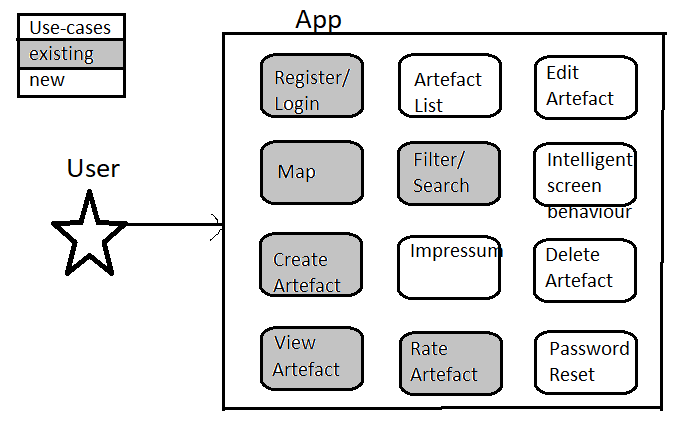
\includegraphics[width=0.8\textwidth]{design/design_use_cases.png}
	\caption{User use-cases}
	\label{fig:designUseCases}
\end{figure}

\section{General Structure}
A look at the use-cases occurs that some of them have a relation to each other and some not. One can see that four segments emerge. In order to provide a better understanding, the following UML activity diagram displays an abstract overview (fig. \ref{fig:activity_flow_generall}).

\begin{figure}[H]
	\centering 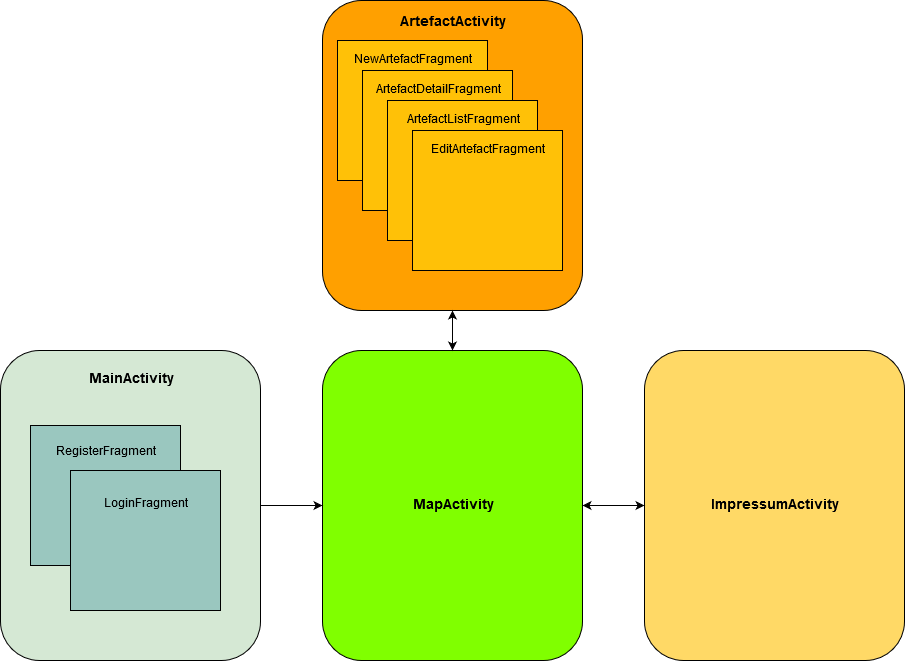
\includegraphics[width=0.8\textwidth]{design/civitas_activity_flow.png}
	\caption{Activity flow diagram}
	\label{fig:activity_flow_generall}
\end{figure}

From here, it is going into detail, and the use-cases are described in their respective activity segments.

% #################################### USER START #####################################

\section{User Management}
The user segment is built within the MainActivity with its belonging Fragments. In here, one should do all events related to the user, like register, login, and request a password reset. As one can see (fig. \ref{fig:activity_flow_generall}), the MainActivity contains the RegisterFragment. This is the home of the user registration process and leads to the corresponding use-case.

\subsection{User Register}
Likewise to the previous version of the Civitas app, this one must have a register/login function as well. Registering to an app is a kind of a weight up. On the one hand it promotes user loyalty to the app; on the other hand, it can be annoying. Even though there is a requirement for registration, it should be simple.
Fortunately, the BaaS by Backendless provides a pleasant way, how this demand can be realized. First of all, one has to characterize what a \textbf{Civitas} user should look like. A user should provide the following properties:
\begin{itemize}
\item name
\item email
\item password
\end{itemize}
This list is extendable by various properties later if additional demands occur. For now, name, email and password are sufficient and build an object of the BackendlessUser.class (fig. \ref{fig:design_user_class_diagram}). 

\begin{figure}[H]
	\centering 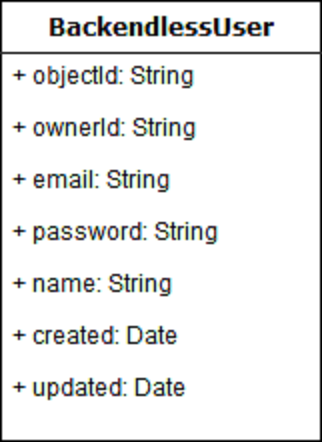
\includegraphics[width=0.5\textwidth]{design/design_user_class_diagram.png}
	\caption{User class diagram}
	\label{fig:design_user_class_diagram}
\end{figure}

The values for created, updated, objectId, and ownerId will be generated automatically if the Backendless request is successful. For lack of space the getter/setter methods of this class are not listed. The complete registration process is displayed in the following listing (list. \ref{code:backendless_register}).

\fbox{
\lstinputlisting[label={code:backendless_register} ,caption={Backendless user registration}, language = java,  numbers = left]{program/backendless_register.java}
}

Passing a user object as an argument to the Backendless.Userservice.register() method is all that needs to be done. Due to the structural behaviour of requesting an interaction with the back-end, and the term of usability stated in the analysis section, one has to pass an asyncCallback handler as the second argument. This asyncCallback requires the implementation of two interface methods. Asynchronous tasks are essential within Android app development. It means the operation performs on the background thread and the leaves the UI thread untouched. This avoids freezing the app and increases the user experience. There is another important effect using the asyncCallback: it offers a smart way to inform the user about the current app status. As long as to whether the handleResponse() or handleFault() method is called, a progress indicator is active, and a fitting message is posted to the user. Hence, one avoids leaving the user waiting for uncertain progress. This pattern is used all across the app.
The following timing diagram (fig. \ref{fig:designRegister}) displays the registration process once again.

\begin{figure}[H]
	\centering 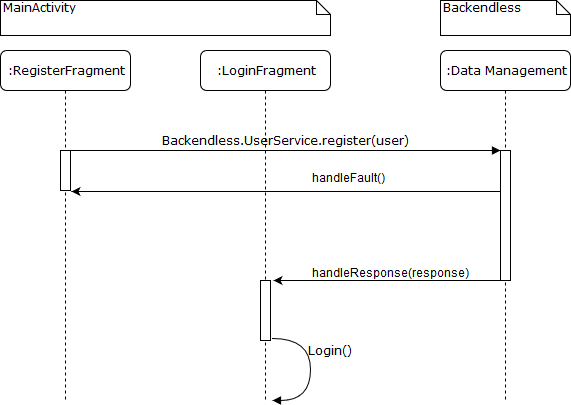
\includegraphics[width=0.8\textwidth]{design/design_register.png}
	\caption{Register timing diagram}
	\label{fig:designRegister}
\end{figure}

\subsection{User Login}
After successful registration, the user should be able to log in. The login process is quite similar to the registration process. Previously registered email and password are the necessary login credentials.
Once a user is logged in, he remains logged in until he logs out. In case of a successful login, the user retrieves all artefact objects stored in the back-end. 

\fbox{
\lstinputlisting[label={code:backendless_login} ,caption={Backendless user login},captionpos=b, language = java,  numbers = left]{program/backendless_login.java}
}



Figure (\ref{fig:designLogin}) visualizes the login process. 
% TODO image erweitern, artefact retreive erläutern.

\begin{figure}[H]
	\centering 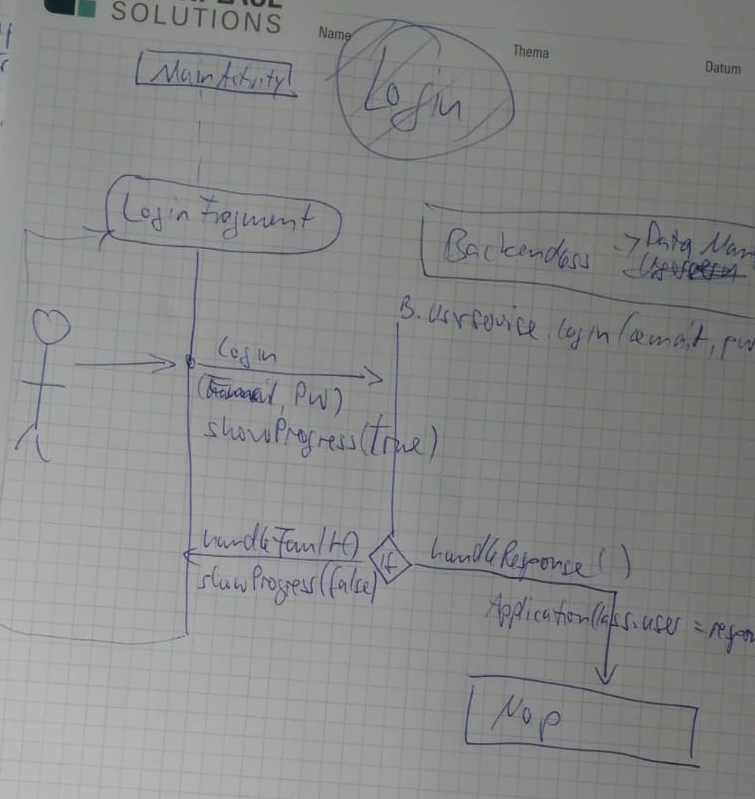
\includegraphics[width=0.8\textwidth]{design/design_login.png}
	\caption{Login timing diagram}
	\label{fig:designLogin}
\end{figure}

Every journey starts with the first step, in this case, with the initial artefact. Due to the development process, there will always be a dummy artefact stored within the database, and one can assume that a multi-user application will not have an empty artefact database. However, two new topics need to be discussed in detail: 1. \textbf{artefacts} and 2. \textbf{retreiving them from the back-end}.
Due to the order of events, retrieving artefacts will be explained next. The artefact will be introduced right on further within the artefact management section.

Successful login triggers the retrieveArtefactsFromBackendless() method. The intention of the Civitas app to manage a growing artefacts database. Therefore it is economically to select the artefacts by certain criteria, like the distance to the mobile device. Backendless provides methods to realize such a selection. Unfortunately, at the time this document is written, and due to a lack of time, the current version generally picks the first 25 data objects (artefacts) from the back-end and returns it to the Civitas app. 
However, to retrieve data objects, one has to create a DataQueryBuilder object and define property settings like page size and offset. Once this is done, one calls the Backendless.Data.of(Artefact.class).find() method and pass the DataQueryBuilder object as an argument to access the artefacts table, where all artefact objects are stored.


Due to the limitation of one million Backendless API calls within the free billing plan, one tries to reduce these calls. To approximate this goal, the ApplicationClass comes into play again. One sets the argument of the handleResponse() method to the ApplicationClass.mArtefactList variable. Doing this stores the data in the cache, so it is also useful in case of bad internet connection.

\subsection{Reset Password}
Alongside with the user registration and login feature, the user might forgot his login credentials. Therefore a reset password function is required. Fortunatly the Backendless API is prepared for this case. In order to improve the security one has to input the registered email address and request a password reset. Now, Backendless sends an email template with reset instructions. The email contains a link directing the user to a mask with an invite to change password.

\begin{figure}[H]
	\centering 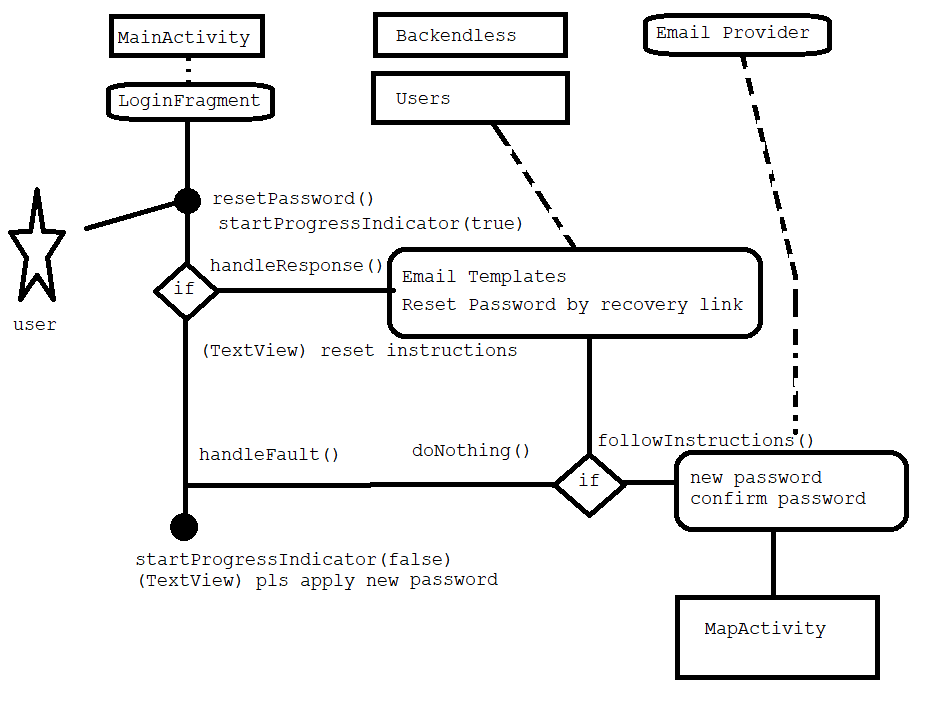
\includegraphics[width=0.8\textwidth]{design/design_reset_password.png}
	\caption{Reset password timing diagram}	
	\label{fig:design_reset_password}
\end{figure} 

% #################################### USER END #####################################

% #################################### MAP START #####################################

\section{Map}
The map view is the point of departure of the Civitas app. In order to indicate the current user position on the map, a permission for the device location must be granted. If the permission is granted the map gets initialized. Consulting \textit{Google APIs for Android} gives the following statement for the usage of the GoogleMap.

\begin{quote}
"This is the main class of the Google Maps SDK for Android and is the entry point for all methods related to the map. You cannot instantiate a GoogleMap object directly, rather, you must obtain one from the getMapAsync() method on a MapFragment... 
Note: Similar to a View object, a GoogleMap can only be read and modified from the Android UI thread. Calling GoogleMap methods from another thread will result in an exception. You can adjust the viewpoint of a map by changing the position of the camera (as opposed to moving the map). You can use the map's camera to set parameters such as location, zoom level, tilt angle, and bearing. For more information, see Camera and View." \cite{googleMap}
\end{quote}

All map related features must be implemented into the onMapReady() method within the getMapAsync() method. It offers one of two possibilities to explore the artefacts within the Civitas app. Depending on which settings are enabled, the map gets populated with markers. One has to seperate three cases, initial entering the map (no settings enabled), entering via navigation drawer, and entering from artefact list overview. The following listing (list. \ref{code:design_map_create_marker}) displays the marker creation process. 

\fbox{
\lstinputlisting[label={code:design_map_create_marker} ,caption={Creating marker within onMapReady()},captionpos=b, style=MeinStyle, numbers = left]{program/design_map_create_marker.java}
}


The other possibility is provided by the artefact list overview and will be introduced later.

Since the artefact objects are stored within the ApplicationClass.mArtefactlist object one does not have to request the back-end to explore the artefacts on the map. 
An artefact will be represented by a custom marker depending on the artefact category. A click on the marker will open an info window for a brief overview. If the user tap on the info window the Civitas app will navigate to a screen for a detailed artefact presentation. This process is displayed in listing (\ref{code:design_map_info_window}).

\fbox{
\lstinputlisting[label={code:design_map_create_marker} ,caption={Marker with info window within onMapReady()},captionpos=b, style=MeinStyle, numbers = left]{program/design_map_info_window.java}
}


% #################################### MAP END #####################################

% #################################### ARTEFACT START #####################################
% TODO: vllt zuerst Map view erklären -> mit dierks besprechen
\section{Artefact Management}
One of the most complex actions the Civitas app will perform is related to the artefacts. There are several opportunities available to the user and they are embedded within the ArtefactActivity (see Diagram \ref{fig:activity_flow_generall}). 

As long as a journey starts with the first step, the artefact section begins with the creation of an artefact and its use-case.

\subsection{Create Artefact}
Entering the map allows the user to create artefacts. A lot of words where written about artefacts in this document. Now it is time to scope out, what is an artefact. In general \textit{"an artefact is an ornament, tool, or other object that is made by a human being, especially one that is historically or culturally interesting."} \cite{artefact}. In the context of this application an artefact is represented by a data object from the Artefact.class. Several properties are mandatory for a new artefact. It must contain a name, description, age, category, and an image. In order to select an image, the user must grant the belonging permission. Capturing a picture with the camera requests the camera permission, choosing one from the gallery requires the permission for reading the external storage. Additionally it can have an audio description. In this case the permission for writing to the external storage and and audio recording must be granted. 
The other properties, such as coordinates and creation date, were generated on the fly during the upload process. Likewise to the BackendlessUser.class diagram, the getter/setter methods are not displayed. The UML class diagram is displayed below (fig. \ref{fig:design_artefact_class_diagram}).

\begin{figure}[H]
	\centering 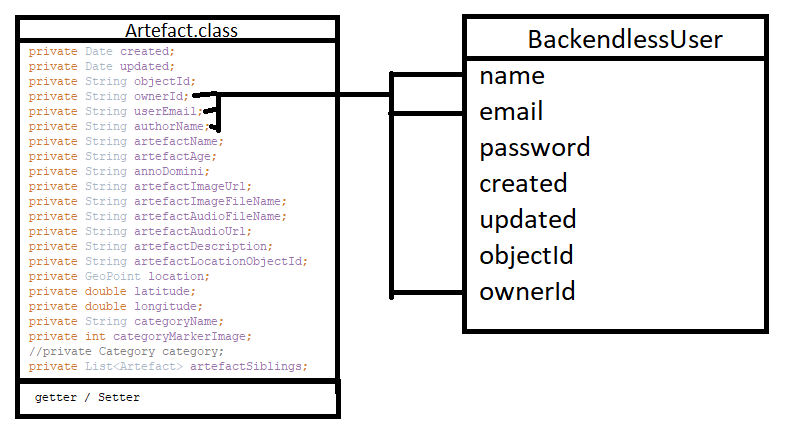
\includegraphics[width=0.8\textwidth]{design/design_artefact_class_diagram.png}
	\caption{Artefact class diagram}	
	\label{fig:design_artefact_class_diagram}
\end{figure}

The creation process is split into different steps, depending on if an audio record is taken or not. Here is a brief overview of the creation steps. 

\begin{table}[h]
\centering
\begin{tabular}{|l|l|l|}
\hline
\textbf{Order} & \textbf{Task} & \textbf{Backendless section} \\ \hline
1.             & uploadImage   & Files                        \\ \hline
2.             & uploadAudio   & Files                        \\ \hline
3.             & saveGeoPoint  & Geolocation                  \\ \hline
4.             & saveArtefact  & Data Management              \\ \hline
\end{tabular}
\caption{Create artefact}
\label{table:create_artefact}
\end{table}

Table (\ref{table:create_artefact}) is visualized by the following UML sequenze diagram (fig. \ref{fig:design_create_artefact}).

\begin{figure}[H]
	\centering 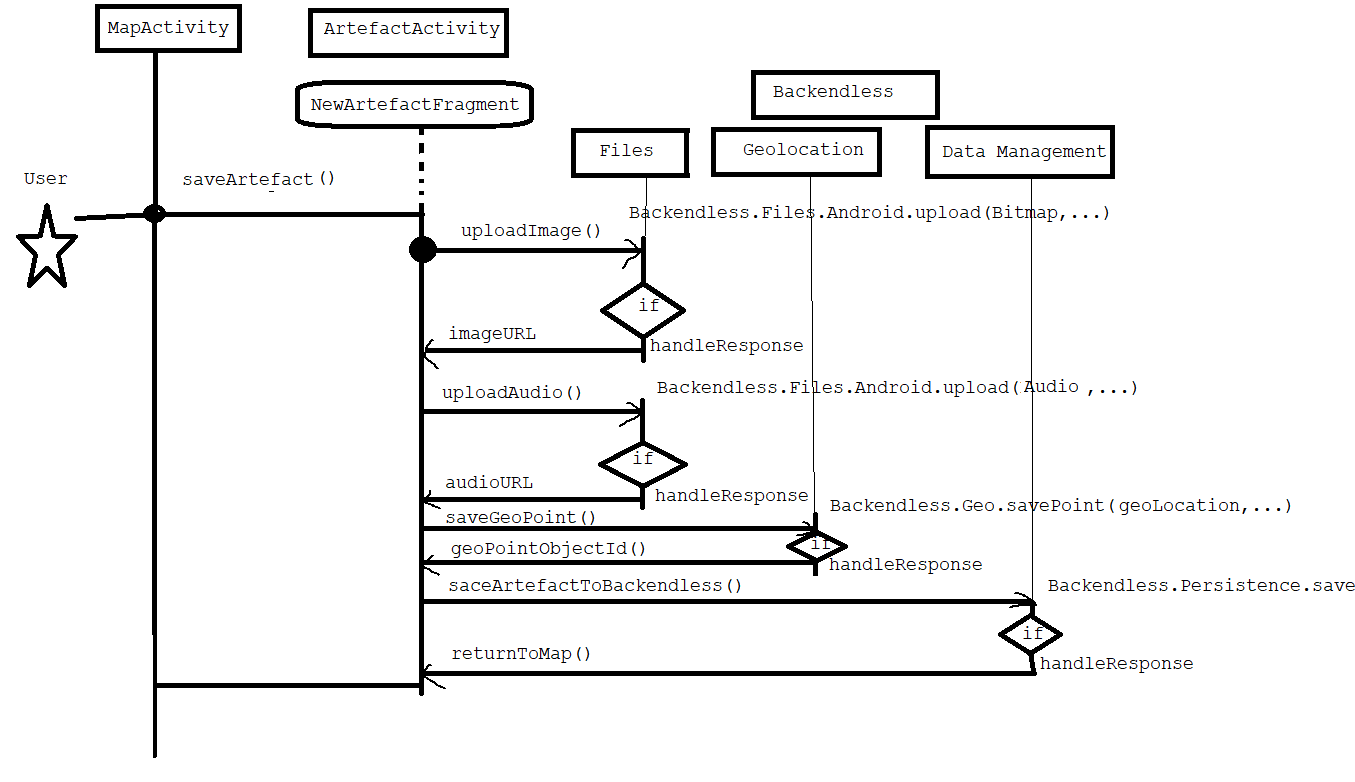
\includegraphics[width=0.8\textwidth]{design/design_create_artefact.png}
	\caption[Design create artefact]{Design create artefact}	
	\label{fig:design_create_artefact}
\end{figure}

Each step build up a connection to the back-end. The back-end returns different responses. The response of step 1. and 2. is an URL, step 3. returns an objectId. These return statements were set with the setter methods of the Artefact.class object to perform step 4.
If the creation sequence is accomplished, one has to update the ApplicationClass variables mArtefactList and mArtefact. Then, the user will be navigated to the location of the newly created artefact on the map. 

There are two possibilities to create an artefact. 
\begin{itemize}
\item[1.] An artefact with the current device location coordinates.
\item[2.] An artefact with the coordinates a onMapLongClick() was performed
\end{itemize}


\subsection{Artefact Detail}
\label{section_artefact_detail}
Hosted in the ArtefactActivity the ArtefactDetailFragment is responsible for a detailed overview. Here is a list of information provided to the user:
\begin{itemize}
\item Artefact name
\item Artefact author
\item Artefact creation date
\item Artefact update date (in case of editting)
\item Artefact category
\item Artefact age
\item Artefact description
\item Artefact image
\end{itemize}

Accessing a selected artefact within the \textbf{ArtefactDetailFragment} for the first time, triggers a back-end request, for displaying the artefact image. Once an image was successfully requested and displayed, it should be stored in the temporary memory cache of the device. Doing this an efficient way to reduce Backendless API calls and increase the performance.
There are two ways to reach the ArtefactDetailFragment. 1. Marker click on the map, 2. Click an artefact from the artefact list overview.

If the user is also the author of the artefact, he is able to edit or delete the artefact.

\subsection{Edit Artefact}
In case of growing knowledge about an artefact, one might will apply changes to that artefact. Within the Civitas app, the user should be able to edit artefacts he has created earlier. Editing is only possible under two conditions. First, the user is at the ArtefactDetailFragment, and second the \textbf{artefactOwnerId} is equal to the current user \textbf{ownerId}\label{subsection:design_delete_artefact}. If those conditions are true, one is justified to edit the artefact. Entering the EditArtefactFragment prepares a copy of the original artefact from the ApplicationClass, to avoid data leaks, in case of abborting the edit process. 
Editing an artefact is even more complex then creating one. Assuming the user will edit an existing artefact, he will be able to change several values, except the location value. 
One has to check which data has changed, and perform the correct action. In the end, it is easier to delete the old artefact data and recreate a new one with the changed values. 
The following table (\ref{table:design_edit_artefact}) gives an abstract overview about the necessary steps and the order in which they are processed.

\begin{table}[h]
\centering
\begin{tabular}{|l|l|}
\hline
\multicolumn{2}{|c|}{\textbf{Edit Artefact}}                                                                                      \\ \hline
1  & ApplicationClass.mArtefactList.remove(mOriginalArtefact)                                                                     \\ \hline
2  & Backendless.Files.remove(imageFilePath, ...)                                                                                 \\ \hline
3  & Backendless.Files.Android.upload(artefactBitmap, ...)                                                                        \\ \hline
3a & mEditArtefact.setArtefactImageUrl(response)                                                                                  \\ \hline
4  & Backendless.Files.remove(audioFilePath, ...)                                                                                 \\ \hline
5  & Backendless.Files.Android.upload(artefactAudioFile, ...)                                                                     \\ \hline
5a & mEditArtefact.setArtefactAudioUrl(response)                                                                                  \\ \hline
6  & Backendless.Persistence.save(mEditArtefact, ...)                                                                             \\ \hline
6a & \begin{tabular}[c]{@{}l@{}}ApplicationClass.mArtefactList.add(response)\\ ApplicationClass.mArtefact = response\end{tabular} \\ \hline
\end{tabular}
\label{table:design_edit_artefact}
\caption{Edit artefact process}
\end{table}


At the end one has to update the ApplicationClass variables again.

Beside the differences between creating and editing an artefact, it is nearly the same process. Therfore, one can reference to figure (\ref{fig:design_create_artefact}) and proceed without a timing diagram of the edit process to the next use-case.


\subsection{Delete Artefact}
Sometimes one wants to delete own artefacts. Therefore, the user should be able to do so. Likewise to the editing process, deleting an artefact is only possible if the same conditions are true. Since an artefact contains an image file, an audio file (optional), a geolocation, and the information content, one has to remove these entries from the back-end. To avoid deleting data by accident, the user should confirm the remove request. A common way to ensure a user confirmation, is providing an alert dialog pop-up window. As long as the removal is in process, the user gets information about the current status. The following UML sequence diagram (fig. \ref{fig:design_delete_artefact}) pictures the removal procress. 

\begin{figure}[H]
	\centering 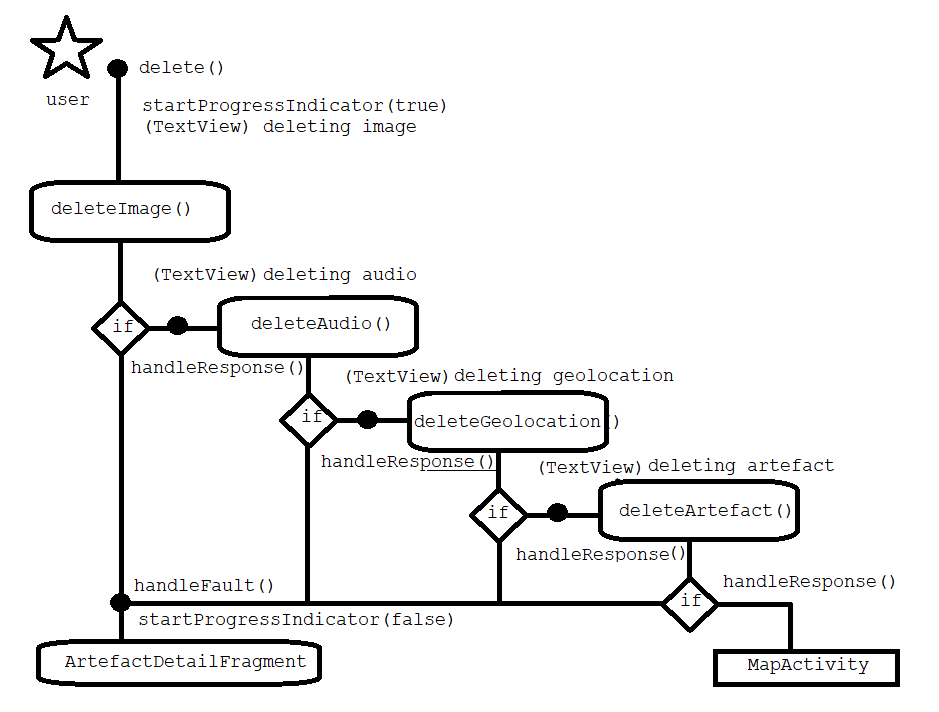
\includegraphics[width=0.8\textwidth]{design/design_delete_artefact.png}
	\caption[Design delete artefact]{Design delete artefact}	
	\label{fig:design_delete_artefact}
\end{figure}


\subsection{Rate Artefact}
A rating system for artefacts is welcomed for multiple purposes. It adds an interactive element to the app and delivers data about quality and credibility of an artefact. As long as the user has not rate an artefact, he is invited to do so. Once he did, only the rating average should be visible. It should be hosted by the \textbf{ArtefactDetailFragment}, but the average should also be visible in each item of the artefact list overview.
Due to a lack of time, it was not possible to implement an artefact rating system. So it is recommended to add such a feature during the next development cycle.

\subsection{Artefact List Overview}

As the predecessor suggests, a user should be able to access a list of his own artefacts. Reconsidering this demands leads to the idea of providing a list of artefacts independetly from the ownership. There are numerous applications within the Google Play Store which provides item list overviews. Therefore, it is obvious to orient on one of them. After analysing the demands, an artefact item within the list should contain the following artefact informations: image, name, category. It is up to the next developer to extend or rearange these properties.

To built and display lists with items several components come together. A list element that contains the data, here an ArrayList<Artefacts> for objects of the artefact class. Further, a view element that displays the data, in this case a RecyclerView object. Finally, an adapter that combines the previous elements. In contrast to the ListView, the RecyclerView has no predefined adapter, so one has to create a custom adapter. At the first glance this might be difficult, but in this way the app benefits from the performance advanteges of the RecyclerView. A ListView creates its items each time it gets visible and destroys them when it disappears, this results in a laggy performance. A RecyclerView binds the items to ViewHolder objects and reference to them. This increases the performance. 
The adapter handles the data from the list and binds them to the views. Therefore, the layout of a single item must be designed within an .xml file. In this case an item is integrated into a CardView element. \textit{"A card view is a type of frame layout that lets you display information on virtual cards. Card views can have rounded corners and shadows to make it look as though they're positioned above their background."} \citep[p. 542]{Griffiths:2017}
Within the card view any view of choice can be displayed. The textual informations are connected to the right TextViews. Usually, one can display an image within an ImageView, if the image is stored in the project. In the Civitas app, the artefacts are stored within the back-end and the artefact contains a URL to its image. With the help of the third-party library Glide one can download and display images from the internet by calling the URL. Glide provides a large amount of options. Currently Glide returns a callback after the first download and caches the images afterwards. This offers the opportunity to inform the user about the progress and reduces the Backendless API calls at the same time. How the elements are put together is displayed in the following listing (\ref{code:design_adapter}).

\fbox{
\lstinputlisting[label={code:design_adapter} ,caption={Impressum},captionpos=b, style=MeinStyle, numbers = left]{program/design_adapter.java}
}

If the user tap on an artefact item the application should launch the belonging detailed artefact view (see section \ref{section_artefact_detail}). To fulfil the predecessors suggestion on should set a filter attribute to display only the artefact items of the current user. It is imaginable to provide several filter attributes to the user. The filter function will be introduced in the following section.


% #################################### ARTEFACT END #####################################

% #################################### IMPRESSUM START #####################################

\section{Imprint}
% Impressumspflicht
Apps are subject to the Telemedia Act (TMG). The TMG prescribes the imprint obligation for apps. Hence, the Civitas app needs an imprint. \textit{"If an Application make content available to the user, then they are to be assigned to the information and communication services... Therfore, an impressum is mandatory."} \cite{impressum}
Due to the fact that the Civitas app provides content to the user one has to implement an impressum. 
Likewise to the MapActivity the Impressum has its own ImpressumActivity with no Fragments. This acitivty contains an WebView element. WebViews can display a website within an Android Application. In this case the user will be guided to the Civitas website. If the user wants to interact with provided content from the website, have to enable the JavaScript settings of the WebView (see Listing \ref{code:impressum}).

\fbox{
\lstinputlisting[label={code:impressum} ,caption={Impressum},captionpos=b, style=MeinStyle, numbers = left]{program/impressum.java}
}

Now, with all these settings enabled the WebView responds to clicks and is able to play videos.

% #################################### IMPRESSUM END #####################################

% #################################### COMMON START #####################################

\section{Common}
Some use-cases wont fit into the four segments, they are touching more of them, or have a generall character. These use-cases will be introduced here.

\subsection{Filter/Search Map/List}
Assuming the Civitas app will contain thousands of artefacts it is very confusing and annoying to discover them without a suitable filtering system. Hence, a user should be able to set certain filter, to display only the artefact items from interest. The previous Civitas app could filter for a selected artefact category and a fixed period of time, e.g. first half of second century before Christ. There is one major reason why this is unsatisfying. The user can not request all artefacts since/until a selected date. Furthermore, the user should be able to view the filtered artefacts whether he is on the map or the artefact list overview and vice versa. Once a filter parameter is set it should stay valid until the user resets the parameter indepently if he leaves map or artefact list overview for a detailed artefact view. Fortunatly the ApplicationClass.mArtefactList contains all available artefacts the filtering process can be realized without any back-end request. The following UML activity chart diagram displays the filter function \ref{fig:design_filter}.

\begin{figure}[H]
	\centering 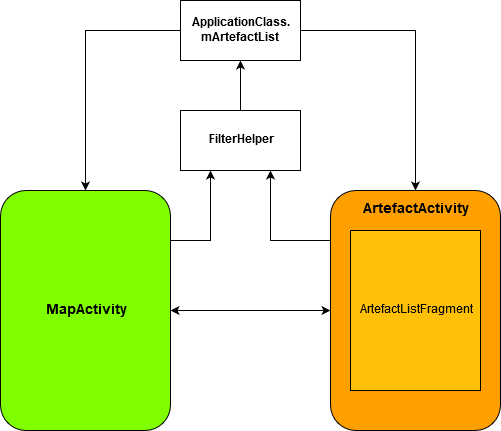
\includegraphics[width=0.8\textwidth]{design/design_filter.png}
	\caption{Filter activity diagram}	
	\label{fig:design_filter}
\end{figure}
Figure (\ref{fig:design_filter}) has only one unknown so far. The FilterHelper.class is built with the singleton pattern. This pattern ensures, that only one instance of this class can be instantiated. This instance is availabe whether the MapActivity or the ArtefactActivity is in focus. Manipulating filter settings within one of these saves the settings for the other and vice versa. The usage of singleton classes should be well considered. Beside advantages like easy usage, access control, they got disadvantages like intransparency and an excessive usage would end up in procedural programming, which is the oposite of object oriented programming. However, in this case it seems to be legit. Since the filtering is a complex operation it will be examined within the test section.
 
Within the Civitas App the user should have the possibility to search certain artefacts by its name. According to the advice of implementing a search field this is realized only within the ArtefactListFragment. This is mainly reasoned by a criteria of usability and the fundamental structure of listing items within Android programming. Displaying items within a list provides certain sorting properties to the developer. A more detailed explaination will follow within the realization chapter (see Chapter \ref{cap:Realization}). These properties allows the user a so called lifesearch for the artefact name value. If the user start typing the fitting results were displayed almost instantly and are way more significant with a belonging image, name, and category rather than a marker representing the category on the map.



\subsection{User Information}
While the Civitas app perform operations in the background, like requesting the back-end, it is possible that the user has to wait until the request is done. To avoid a so called app freeze, all operations should be done in a asynchronous way. In order to increase the user experience the Civitas app should indicate the user that an operation is in progress and what kind of operation is currently performed. Once an operation is accomplished the progress indicator should be disappear. A generalized user information flow is displayed in the following image (see \ref{fig:design_user_information}).

\begin{figure}[H]
	\centering 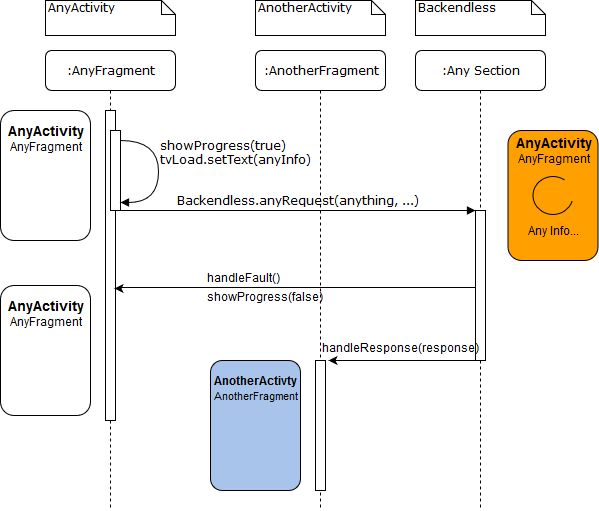
\includegraphics[width=0.8\textwidth]{design/design_user_information.png}
	\caption{User information timing diagram}	
	\label{fig:design_user_information}
\end{figure}


\subsection{Screen Focus}
Another aspect to increase the user experience is tied to the screen behaviour after (re-)entering the map. The previous Civitas app screen always returns to the current device location whether one views the details of an artefact within close or wide range. It turns out that this is annoying, when e.g. one is localized in Hamburg and will discover the artefacts in the area of Rome. Therefore it is mandatory to save the coordinates of the area the screen is focussed on. There are several subtle cases, when the coordinates are not so obvious available. The following table displays which cases are taken into account for a corresponding screen position (tab. \ref{table:screen_focus}).

\begin{table}[H]
\centering
\begin{tabular}{|l|l|}
\hline
\textbf{Case}                                                                                               & \textbf{Screen Position}         \\ \hline
Initial entering the map                                                                                    & Device location                  \\ \hline
\begin{tabular}[c]{@{}l@{}}Re-enter the map from \\ DetailArtefactFragment\end{tabular}                     & Artefact location                \\ \hline
\begin{tabular}[c]{@{}l@{}}Re-enter the map from \\ ArtefactListFragment\end{tabular}                       & Last screen position             \\ \hline
\begin{tabular}[c]{@{}l@{}}Re-enter the map with \\ active filter from \\ ArtefactListFragment\end{tabular} & Device location                  \\ \hline
\begin{tabular}[c]{@{}l@{}}Re-enter the map from \\ NewArtefactFragment\end{tabular}                        & Artefact location                \\ \hline
\begin{tabular}[c]{@{}l@{}}Re-enter the map from \\ EditArtefactFragment\end{tabular}                       & Artefact location                \\ \hline
\begin{tabular}[c]{@{}l@{}}Re-enter the map after \\ deleting an artefact\end{tabular}                      & Location of the deleted artefact \\ \hline
\begin{tabular}[c]{@{}l@{}}Re-enter the map from \\ ImpressumActivity\end{tabular}                          & Last screen position             \\ \hline
default                                                                                                     & Device location                  \\ \hline
\end{tabular}
\caption{Screen focus behaviour by certain events}
\label{table:screen_focus}
\end{table}

Depending on the listed cases the current screen position get captured with the following method (list. ).

\fbox{
\lstinputlisting[label={code:design_screen_position} ,caption={Capture the current screen position},captionpos=b, style=MeinStyle, numbers = left]{program/design_screen_position.java}
}

The user can return to the device location by tapping the \textbf{Location} Button in the ActionBar.
Moving the screen position with an animation gives the user the feeling to be taken on a journey from an artefact to the device location.

At this point ends the description of the Android application features and it continues with the back-end section. 


%################################################################

\section{Backendless}

Backendless combines two out of three key ingredients of the Civitas project. The data storage within a back-end and a web application corresponding to the Android application. It has a huge documentation section for a number a different \textbf{API}s. API is an acronym for \textbf{a}pplication \textbf{p}rogramming \textbf{i}nterface and it defines, how to communicate among various components. In this thesis the Android API is in the scope of interest.

\begin{figure}[H]
	\centering 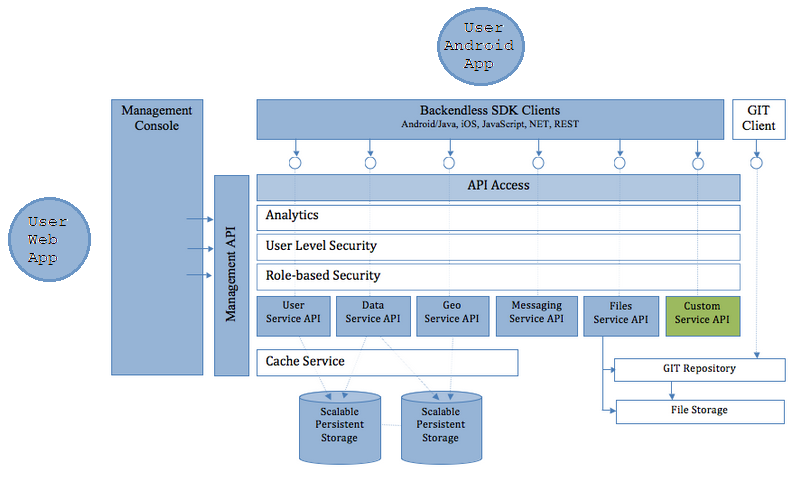
\includegraphics[width=0.8\textwidth]{design/backendless_api_overview.png}
	\caption{Backendless API overview}
	\label{fig:backendless_api_overview}
\end{figure}


Using BaaS simplifies the storage of the app data. Successful back-end request access the Backendless console. Depending on the request the data is stored in the related segment. One can select between synchronous or asynchronous interaction. Synchronous means that interaction is handled on main thread and the app waits until the interaction is accomplished. This can freeze the app, confuses the user and decreases the user experience. To avoid this perfomance leaks, the decision was made to use asynchronous interactions within the Civitas app. Asynchronous operations take place in the background, so the main thread is free. 
Independently of the Java operation that will be performed, Backendless behaves always with the same pattern. If a Backendless request was made, one has to implement two interface callback methods, a) handleResponse() and b) handleFault(). Case a) represents a successful request and delivers the desired object within its argument. Case b) is more or less self-explaining and gives a feedback if something failed.

The first step to connect an Android app with Backendless is to register at https://backendless.com/ and create an app in the dashboard. Once this is done, one has to input the \textbf{Application Id}, \textbf{API key} and \textbf{server url} provided by the Backendless app into the Application class of the Android app (see listing \ref{code:connect_android_backendless}). Adding the dependency to the build.gradle(Module:app) file enables the third party library content of Backendless within the Android app.

\fbox{
\lstinputlisting[label={code:connect_android_backendless} ,caption={Connecting Android app with Backendless},captionpos=b, style=MeinStyle, numbers = left]{program/backendless_app_initializing.java}
}

After everything is setup successfully, it is time to discuss the benefits Backendless delivers to the Civitas project.

\subsection{Back-end}
The back-end is used to store user informations and the artefact data. The user informations are pretty straight forward containing only string values for certain properties. The artefact data is more complex, while it is a combination of files, geolocation and string values. Therefore, one has to access different sections within the Backendless console. The string values of the users and the artefacts were stored in the belonging tables within the Data Management section. The artefact files were stored in the Files section, and the artefact geolocation within the Geolocation section.



\subsection{Civitas - Web App}
As an advice from the predecessor an admin control panal was mentioned. Using BaaS from Backendless delivers a web application which can be treated as an admin control panel. Primarily the admin control panel should fulfil functions to maintain the Civitas data set. 

\subsection{Admin Use Cases}

Since the web app is included within the BaaS it was unnecessary to care about the design during the Civitas project. Anyway, an explaination will follow here.
At this point of development process, the \textbf{Civitas} project handles data about users and artefacts. Therefore, the following admin use-cases are determined:
\begin{itemize}
\item Statistics
\item Maintain Data
\item Files
\item Geolocation
\item Mail Services
\end{itemize}

Within the admin control panel the Civitas admin has a large selection to maintain the user, and artefact data. The fitting Backendless API makes it easy to handle data object tables, user credentials, password recovery, file transfers, mail service, and geolocation operations within a clear presentation. Visualizing the adimg use-cases is the best way to provide an impression of the admin control panel is.

\subsubsection*{Statistics}
The app credentials were and several statistics are available within the dashboard (fig \ref{fig:backendless_console_main_overview}). From here, on can discover the other functions of Backendless.

\begin{figure}[H]
	\centering 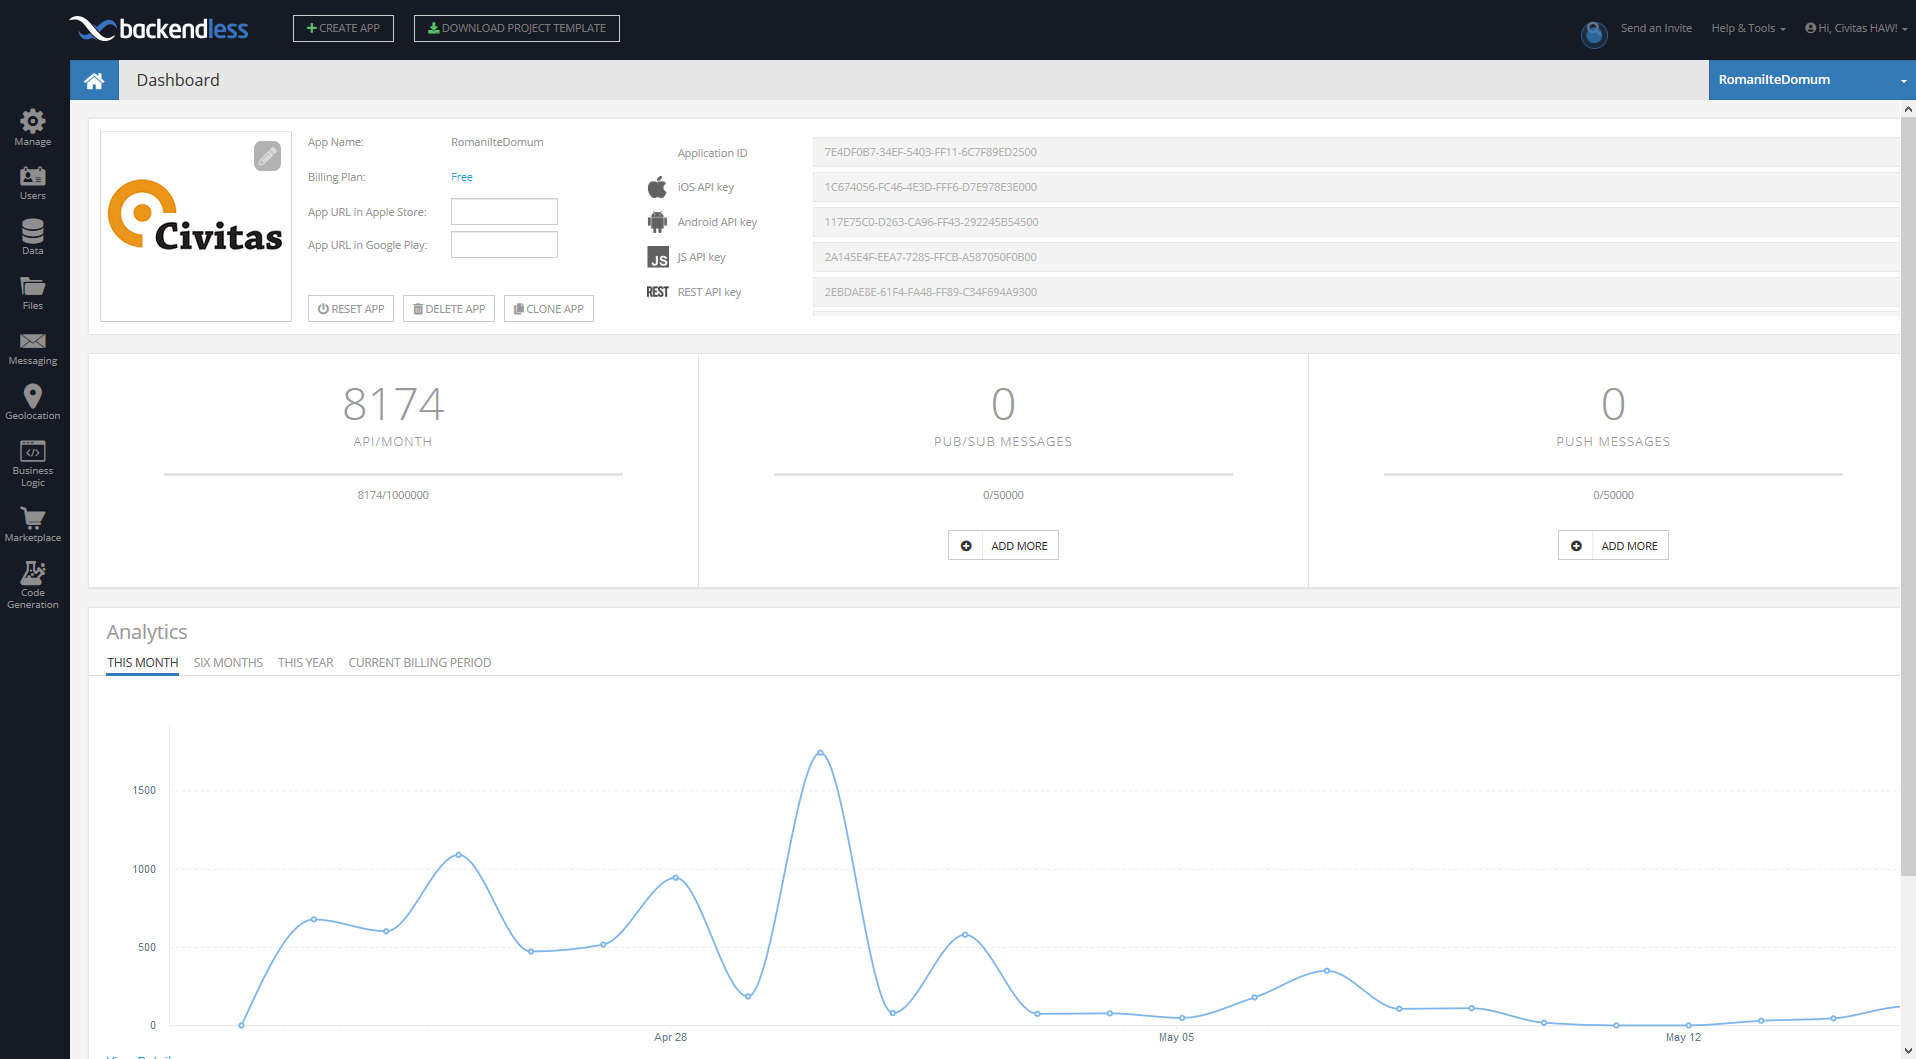
\includegraphics[width=0.8\textwidth]{design/backendless_console_main_overview.png}
	\caption{Admin control panel dashboard}
	\label{fig:backendless_console_main_overview}
\end{figure}


\subsubsection*{Maintain Data}
All data, whether user or artefact, are displayed in the data management section. Several different views and operations are available from manipulating a single value within an artefact to deleting the complete artefact table (fig. \ref{fig:backendless_console_artefact_table}).
\begin{figure}[H]
	\centering 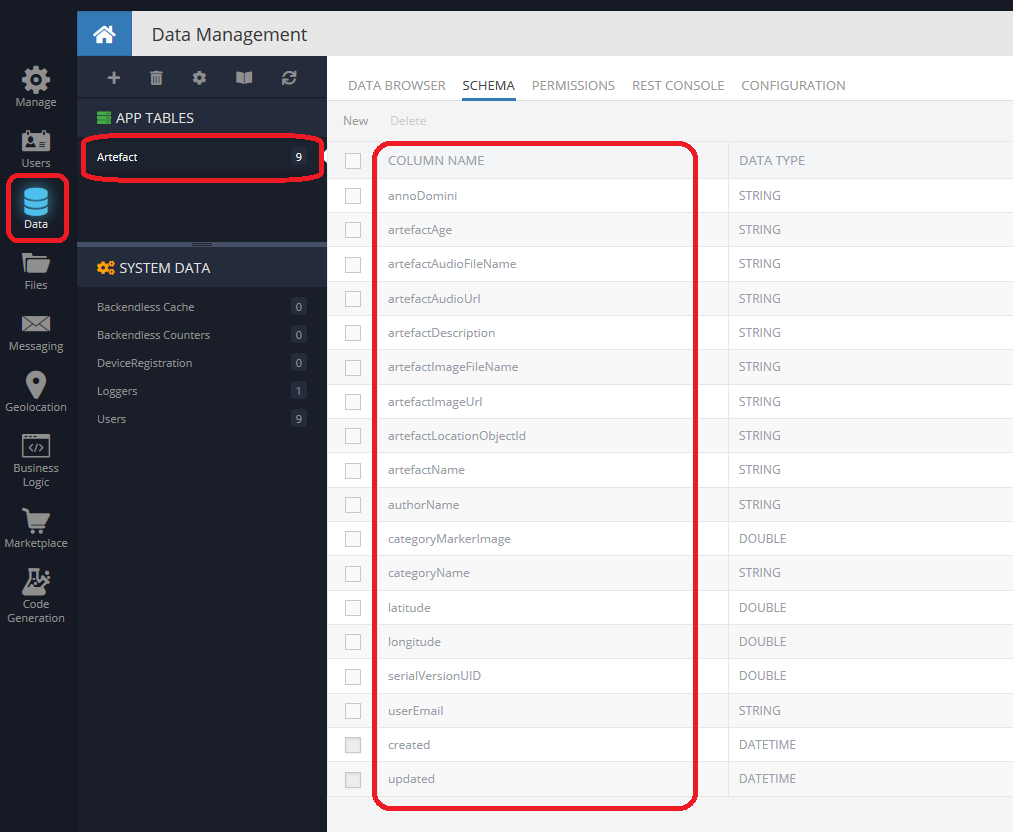
\includegraphics[width=0.8\textwidth]{design/backendless_console_artefact_table.png}
	\caption{Admin control panel data management}
	\label{fig:backendless_console_artefact_table}
\end{figure}

\subsubsection*{Files}
Uploaded files will be stored in the Backendless files section. In this case, the files are seperated in image and audio files folders.  Figure (\ref{fig:backendless_console_files}) displays the storage of the artefact image files. 

\begin{figure}[H]
	\centering 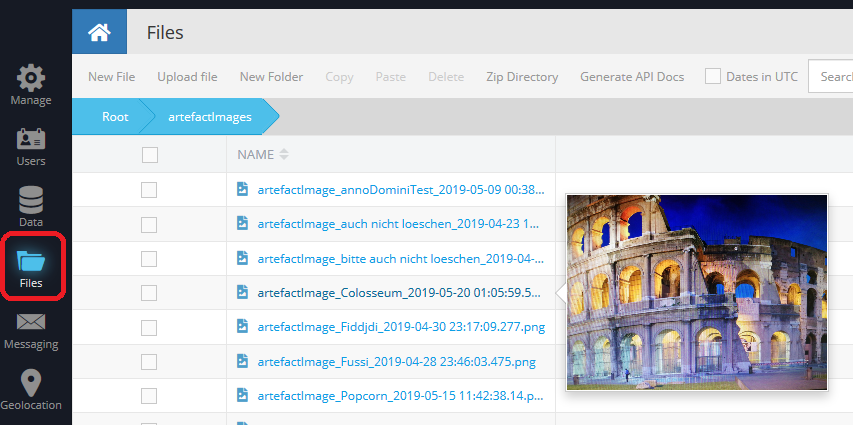
\includegraphics[width=0.8\textwidth]{design/backendless_console_files.png}
	\caption{Admin control panel files section}
	\label{fig:backendless_console_files}
\end{figure}

\subsubsection*{Geolocation}
Artefacts within the Civitas Android app are represented as markers on the map. The same markers are displayed within this geolocation section with the relation to their artefact object. This provides a great overview about the current data set (fig \ref{fig:backendless_geolocation}).

\begin{figure}[H]
	\centering 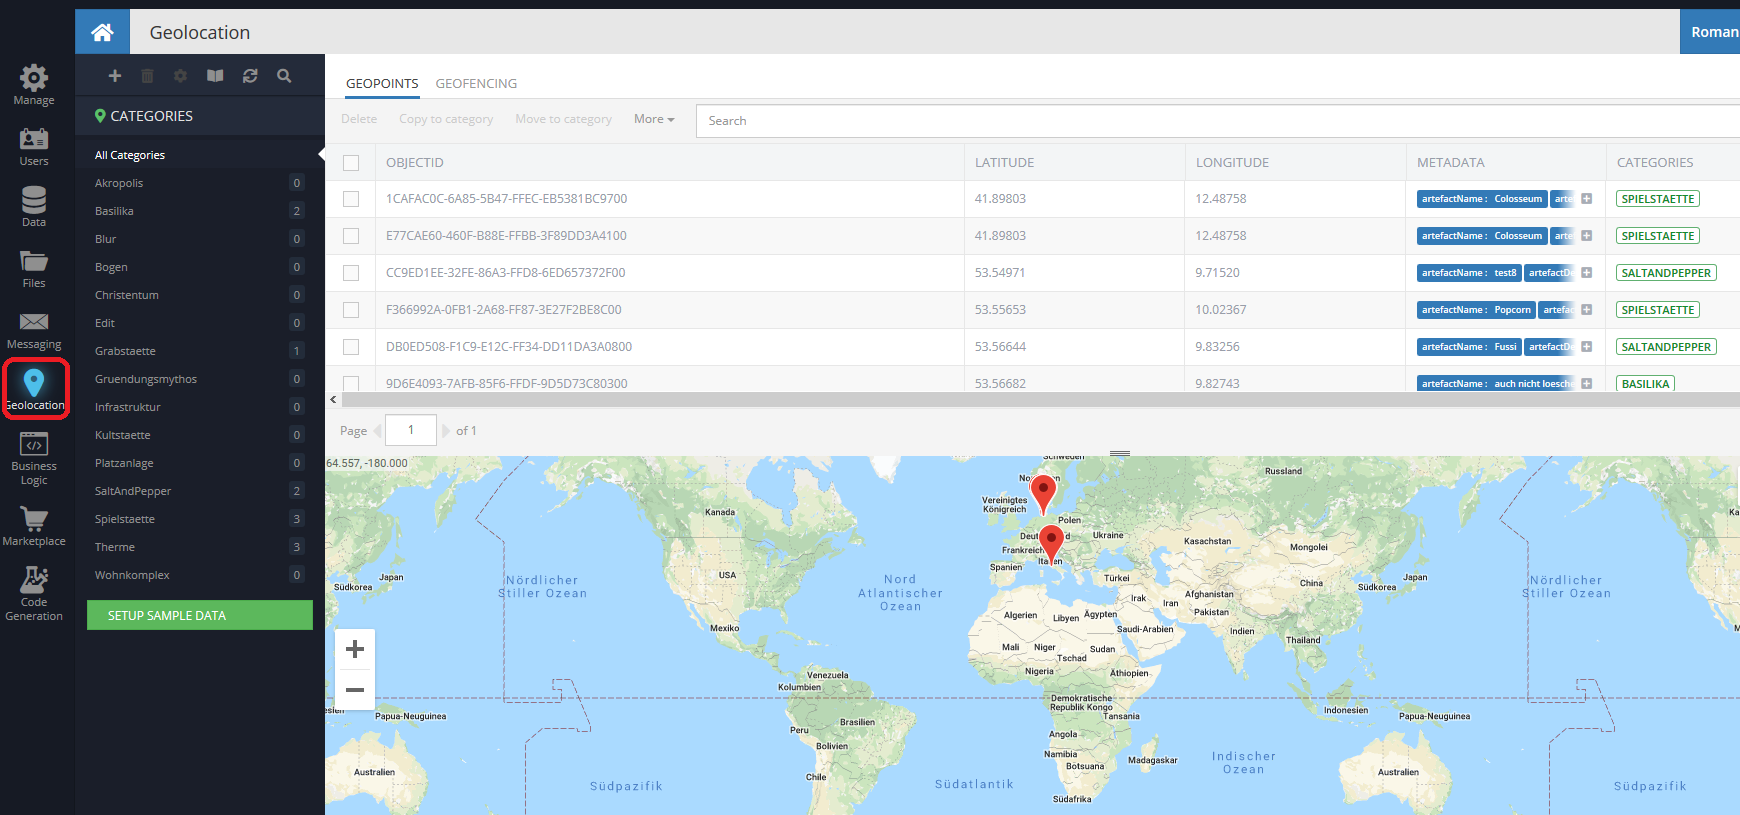
\includegraphics[width=0.8\textwidth]{design/backendless_geolocation.png}
	\caption{Admin control panel geolocation section}
	\label{fig:backendless_geolocation}
\end{figure}

\subsubsection*{Mail Services}
Email templates for a variety of events were provided by Backendless. One can enable/disable the different templates and customize these. Figure (\ref{fig:backendless_email_template}) displays the email template for password recovery.

\begin{figure}[H]
	\centering 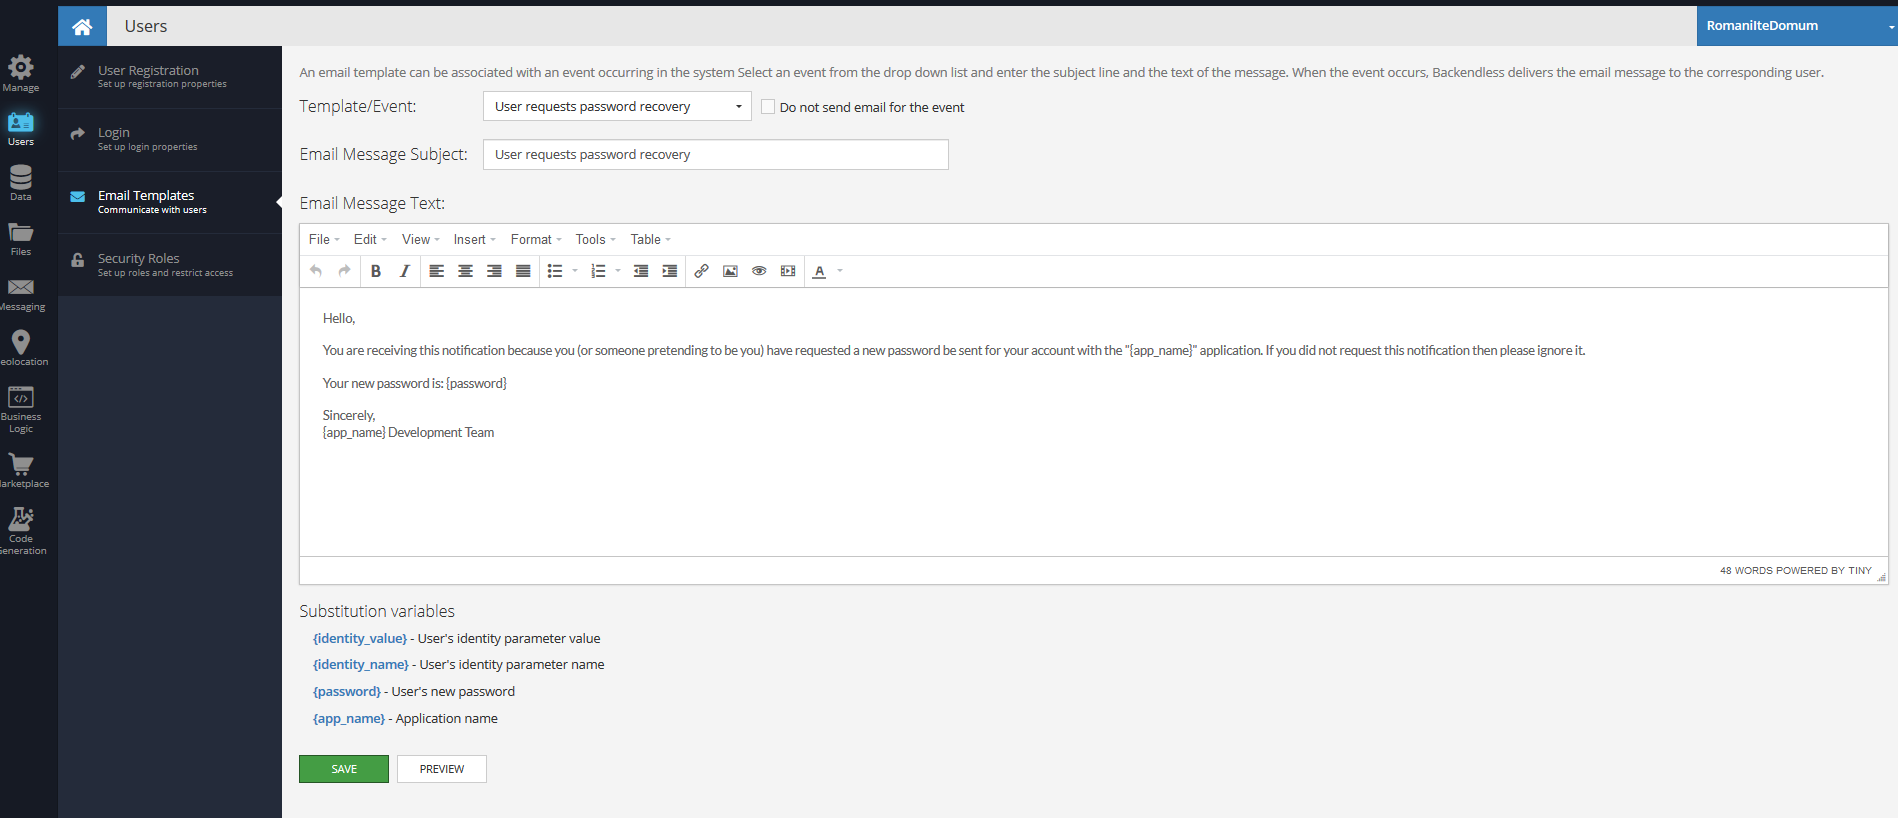
\includegraphics[width=0.8\textwidth]{design/backendless_email_template.png}
	\caption{Admin control panel email template}
	\label{fig:backendless_email_template}
\end{figure}


After finishing the presentation of the admin control panel, the next step is the realization of the Civitas Android app.

